\documentclass{article} % For LaTeX2e
\usepackage{nips14submit_e,times}
\usepackage{hyperref}
\usepackage{url}
\usepackage{amsmath}
\usepackage{amssymb}
\usepackage{amsthm}
\usepackage{mathtools,enumitem}
\usepackage{algorithm}
\usepackage{algorithmic}
%\documentstyle[nips14submit_09,times,art10]{article} % For LaTeX 2.09

\usepackage{tikz}
\usepackage{cite}

% Math operators
\newcommand{\scal}[2]{\left\langle #1 , #2 \right\rangle}
\DeclareMathOperator{\IR}{\mathbb{R}}
\DeclareMathOperator*{\argmin}{argmin}
\DeclareMathOperator{\One}{\mathbbm{1}}
\DeclareMathOperator{\Ccal}{\mathcal{C}}
\DeclareMathOperator{\logsumexp}{logsumexp}
\DeclareMathOperator{\diag}{diag}
\newcommand{\norm}[1]{\left\lVert #1 \right\rVert}
\renewcommand{\epsilon}{\varepsilon}

\theoremstyle{plain}
\newtheorem{theorem}{Theorem}
\newtheorem{proposition}{Proposition}
\newtheorem{lemma}{Lemma}
\newtheorem{corollary}{Corollary}

\theoremstyle{definition}
\newtheorem{definition}{Definition}

\theoremstyle{remark}
\newtheorem{remark}{Remark}
\newtheorem{example}{Example}


\title{Over-relaxed Sinkhorn's Algorithm for Regularized Optimal Transport}

%
\author{
Alexis THIBAULT\\
\'Ecole Normale Sup\'erieure\\
Paris, France\\
\texttt{alexis.thibault@ens.fr}
 \And
L\'enaic CHIZAT\\
\'Ecole Normale Sup\'erieure\\ Paris Dauphine (PSL research University)\\
Paris, France\\
\texttt{lenaic.chizat@ens.fr}
 \AND
Charles DOSSAL\\
INSA Toulouse\\
Institut de Math\'ematiques de Toulouse\\
Toulouse,  France\\
\texttt{dossal@insa-toulouse.fr}
\And 
Nicolas PAPADAKIS\\
CNRS, Institut de Math\'ematiques de Bordeaux\\
Talence, France\\
\texttt{nicolas.papadakis@math.u-bordeaux.fr}
} 
% The \author macro works with any number of authors. There are two commands
% used to separate the names and addresses of multiple authors: \And and \AND.
%
% Using \And between authors leaves it to \LaTeX{} to determine where to break
% the lines. Using \AND forces a linebreak at that point. So, if \LaTeX{}
% puts 3 of 4 authors names on the first line, and the last on the second
% line, try using \AND instead of \And before the third author name.

\newcommand{\fix}{\marginpar{FIX}}
\newcommand{\new}{\marginpar{NEW}}

\nipsfinalcopy % Uncomment for camera-ready version

\begin{document}


\maketitle

\begin{abstract}
This article describes a method for quickly calculating the solution to the regularized optimal transport problem. It generalizes and improves upon the widely-used iterative Bregman projections algorithm (or Sinkhorn's algorithm). The idea is to over-relax the Bregman projection operators, allowing for faster convergence. In practice this corresponds to elevating the diagonal scaling factors to a given power, at each step of the algorithm.
\end{abstract}

\section{Introduction}
Optimal Transport is an efficient and flexible tool to compare two probability distributions which has been popularized in the computer vision community in the context of discrete histograms \cite{Rubner2000}. The introduction of entropic regularization in \cite{cuturi13} has made possible the use of the fast Sinkhorn's algorithm \cite{sinkhorn64}   scaling with high dimensional data. 
Regularized optimal transport have thus been intensively used  in  Machine Learning with applications such as   Geodesic PCA \cite{seguy2015principal}, domain adaptation \cite{2015arXiv150700504C}, data fitting \cite{2015arXiv150605439F},  training of Boltzmann Machine \cite{NIPS2016_6248}  or dictionary learning \cite{Rolet2016,2017arXiv170801955S}.

The computation of optimal transport between two data relies on the estimation of an optimal transport matrix, the entries of which represent the quantity of mass transported between  data locations. 
Regularization of optimal transport with strictly convex regularizers \cite{cuturi13, dessein2016}  nevertheless involves a spreading of the mass. Hence, for particular purposes such as color interpolation \cite{Rabin2014} or gradient flow \cite{2016arXiv160705816C}, it is  necessary  to consider very small regularization of the problem.
In this setting,  the regularized transport problem can be ill-conditioned. This is the issue  we want to tackle here.
Before going into further details, we now briefly introduce the main notations and concepts used all along this article.

 
\subsection{Discrete Optimal Transport}
We consider two discrete probability measures $\mu^k \in \IR_{+*}^{n_k}$.
Let us define the two following linear operators
\begin{align*}
A_1 &: \begin{cases}
\IR^{n_1 n_2} \rightarrow \IR^{n_1} \\
(A_1 x)_i = \sum_j x_{i,j}
\end{cases} &
A_2 &: \begin{cases}
\IR^{n_1 n_2} \rightarrow \IR^{n_2}\\
(A_2 x)_j = \sum_i x_{i,j},
\end{cases}
\end{align*}
as well as the linear  constraint sets
\begin{align*}
\Ccal_k &= \left\{ \gamma\in\IR^{n_1 n_2} \mid A_k \gamma = \mu^k \right\}.
\end{align*}
Given a cost matrix $c$, where $c_{ij}$ represents the cost of moving mass $\mu^1_i$ to $\mu^2_j$,  the optimal transport problem corresponds to the estimation of an optimal transport matrix $\gamma$ solution of:
$$\min_{\gamma\in\Ccal_1\cap \Ccal_2\cap \IR^{n_1 n_2}_+} \langle c,\gamma\rangle:=\sum_{i,j}c_{i,j}\gamma_{i,j}.$$
This is a linear programing problem whose resolution is unmanageable for large scale problems. 

\subsection{Regularized optimal transport}

In \cite{cuturi13}, it has been proposed to regularize this problem by adding a strictly convex entropy regularization:
\begin{equation}\label{ROT}
\min_{\gamma\in\Ccal_1\cap \Ccal_2\cap \IR^{n_1 n_2}_{+*}}K^\epsilon(\gamma) := \scal{c}{\gamma} 
+ \epsilon KL(\gamma,\mathbf{1})
,\end{equation}
with $\epsilon>0$, $\mathbf{1}$ is the matrix of size $n_1\times n_2$ full of ones and the Kullback-Leibler divergence is:
\begin{equation}\label{KL}
KL(\gamma,\xi) = \sum_{i,j} \gamma_{i,j} \left( \log \left( \frac{\gamma_{i,j}}{\xi_{i,j}} \right) -1  \right) + \sum_{i,j} \xi_{i,j}.
\end{equation}
It was shown in \cite{benamou15}  that the regularized optimal transport matrix $\gamma^*$, which is the unique minimizer of problem \eqref{ROT},  is the Bregman projection of $\gamma^0 = e^{-c/\epsilon}$ onto $\Ccal_1 \cap \Ccal_2$:
\begin{equation}\label{eq:reg_ot_pb}
\gamma^* = \argmin_{\Ccal_1 \cap \Ccal_2} K^\epsilon(\gamma)= P_{\Ccal_1 \cap \Ccal_2} (e^{-c/\epsilon}),
\end{equation}
where $P_{\Ccal}$ is the  Bregman projection onto $\Ccal$ defined as:
\[
P_{\Ccal}(\xi) := \argmin_{\gamma \in \Ccal} KL(\gamma,\xi).
\]



\subsection{Sinkhorn's algorithm}
Iterative Bregman projections onto $\Ccal_1$ and $\Ccal_2$ converge to a point in the intersection $\Ccal_1 \cap \Ccal_2$ \cite{bregman67}. Hence, the so-called Sinkhorn algorithm \cite{sinkhorn64} that performs alternate Bregman projections, can be considered to compute the regularized  transport matrix:
\begin{align*}
\gamma^0 &= e^{-c/\epsilon} &
\gamma^{l+1} = P_{\Ccal_2}(P_{\Ccal_1}(\gamma^l)),
\end{align*}
and we have 
$\lim_{l\rightarrow +\infty} \gamma^l = P_{\Ccal_1 \cap \Ccal_2}(\gamma^0) = \gamma^*.$

In the discrete setting,  projections actually correspond to diagonal scalings.
\begin{align}\label{scaling}
P_{\Ccal_1}(\gamma) &= \diag(a) \gamma &
a &=  {\mu^1}\oslash{A_1 \gamma} \\
P_{\Ccal_2}(\gamma) &= \gamma \diag(b) &
b &= {\mu^2}\oslash{A_2 \gamma}\nonumber
\end{align}
where $\oslash$ is the pointwise division. 
To compute numerically the solution  one simply has to store $(a^l, b^l)\in\IR^{n_1+n_2}$ and iterates
\begin{align*}
a^{l+1} &= {\mu^1}\oslash{\gamma^0 b^l} &
b^{l+1} &= {\mu^2}\oslash{^t \gamma^0 a^{l+1}} 
\end{align*}
where the transport matrix can be recovered as :
$\gamma^l = \diag(a^l) \gamma^0 \diag(b^l).$ 
Efficient parallel computations can be considered \cite{cuturi13} and one can even reach real-time computation for large scale problem for certain class of cost matrices $c$ \cite{Solomon2015}. 
For small values of the parameter $\epsilon$, numerical issues can arise and a stabilization of the algorithm is necessary \cite{2016arXiv160705816C}.
The convergence of the process can nevertheless be very slow  in the setting $\epsilon\to 0$.
\subsection{Related works }
The introduction of relaxation variables through heavy ball approaches \cite{POLYAK19641} has recently gained in popularity  to speed up the convergence of algorithms optimizing convex \cite{2014arXiv1412.7457G} or non convex \cite{Zavriev1993,2016arXiv160609070O} problems. Such schemes have also been empirically considered to accelerate Sinkhorn's algorithm  in \cite{peyre2016quantum,2017arXiv170801955S}. The convergence of these algorithms is nevertheless not studied yet in the context of regularized optimal transport.

\subsection{Overview and contributions}
In this paper, we consider an over-relaxation scheme designed to accelerate   Sinkhorn's algorithm. We first present and show the convergence of our algorithm in section 2. In section 3, we analyze the local convergence rate of the algorithm to justify the acceleration.
We finally demonstrate numerically  in Section 4 the good behavior of our method, where larger accelerations are observed for decreasing values of $\epsilon$.



\section{Over-relaxed Sinkhorn's algorithm}

As illustrated in Figure \ref{alternate_projections} (a-b), the Sinkhorn algorithm, that  performs alternate Bregman projections onto the affine sets $\Ccal_1$ and $\Ccal_2$, can be very slow when $\epsilon\to 0$. The idea developped in this paper is to perform over-relaxed projections in order to accelerate the process, as displayed in Figure \ref{alternate_projections} (c) 

\begin{figure}[ht!]
\begin{center}
\begin{tabular}{ccc}
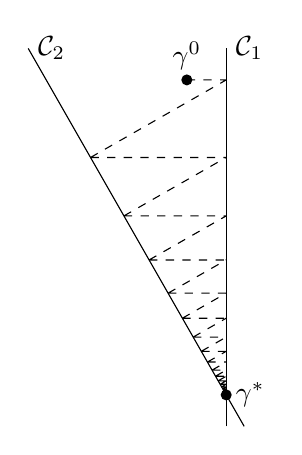
\begin{tikzpicture}
\fill (-0.500000,4.000000) circle (2pt) node[above] (gamma0) {$\gamma^0$};
\fill (0,0) circle (2pt) node[right] {$\gamma^*$};
\draw[dashed] (-0.500000,4.000000) -- (0.000000,4.000000)
(-1.723077,3.015385) -- (0.000000,4.000000)
(-1.723077,3.015385) -- (0.000000,3.015385)
(-1.298935,2.273136) -- (0.000000,3.015385)
(-1.298935,2.273136) -- (0.000000,2.273136)
(-0.979197,1.713595) -- (0.000000,2.273136)
(-0.979197,1.713595) -- (0.000000,1.713595)
(-0.738164,1.291787) -- (0.000000,1.713595)
(-0.738164,1.291787) -- (0.000000,1.291787)
(-0.556462,0.973809) -- (0.000000,1.291787)
(-0.556462,0.973809) -- (0.000000,0.973809)
(-0.419487,0.734102) -- (0.000000,0.973809)
(-0.419487,0.734102) -- (0.000000,0.734102)
(-0.316228,0.553400) -- (0.000000,0.734102)
(-0.316228,0.553400) -- (0.000000,0.553400)
(-0.238388,0.417178) -- (0.000000,0.553400)
(-0.238388,0.417178) -- (0.000000,0.417178)
(-0.179708,0.314488) -- (0.000000,0.417178)
(-0.179708,0.314488) -- (0.000000,0.314488)
(-0.135472,0.237076) -- (0.000000,0.314488)
(-0.135472,0.237076) -- (0.000000,0.237076)
(-0.102125,0.178719) -- (0.000000,0.237076)
(-0.102125,0.178719) -- (0.000000,0.178719)
(-0.076987,0.134726) -- (0.000000,0.178719)
(-0.076987,0.134726) -- (0.000000,0.134726)
(-0.058036,0.101563) -- (0.000000,0.134726)
(-0.058036,0.101563) -- (0.000000,0.101563)
(-0.043750,0.076563) -- (0.000000,0.101563)
(-0.043750,0.076563) -- (0.000000,0.076563)
(-0.032981,0.057717) -- (0.000000,0.076563)
(-0.032981,0.057717) -- (0.000000,0.057717)
(-0.024863,0.043509) -- (0.000000,0.057717)
(-0.024863,0.043509) -- (0.000000,0.043509)
(-0.018743,0.032799) -- (0.000000,0.043509)
(-0.018743,0.032799) -- (0.000000,0.032799)
(-0.014129,0.024726) -- (0.000000,0.032799)
(-0.014129,0.024726) -- (0.000000,0.024726)
(-0.010651,0.018639) -- (0.000000,0.024726)
(-0.010651,0.018639) -- (0.000000,0.018639)
(-0.008029,0.014051) -- (0.000000,0.018639)
(-0.008029,0.014051) -- (0.000000,0.014051)
(-0.006053,0.010592) -- (0.000000,0.014051)
(-0.006053,0.010592) -- (0.000000,0.010592)
(-0.004563,0.007985) -- (0.000000,0.010592)
(-0.004563,0.007985) -- (0.000000,0.007985)
(-0.003440,0.006020) -- (0.000000,0.007985)
(-0.003440,0.006020) -- (0.000000,0.006020)
(-0.002593,0.004538) -- (0.000000,0.006020)
(-0.002593,0.004538) -- (0.000000,0.004538)
(-0.001955,0.003421) -- (0.000000,0.004538)
(-0.001955,0.003421) -- (0.000000,0.003421)
(-0.001474,0.002579) -- (0.000000,0.003421)
(-0.001474,0.002579) -- (0.000000,0.002579)
(-0.001111,0.001944) -- (0.000000,0.002579)
(-0.001111,0.001944) -- (0.000000,0.001944)
(-0.000837,0.001465) -- (0.000000,0.001944)
(-0.000837,0.001465) -- (0.000000,0.001465)
(-0.000631,0.001105) -- (0.000000,0.001465)
(-0.000631,0.001105) -- (0.000000,0.001105)
(-0.000476,0.000833) -- (0.000000,0.001105)
(-0.000476,0.000833) -- (0.000000,0.000833)
(-0.000359,0.000628) -- (0.000000,0.000833)
(-0.000359,0.000628) -- (0.000000,0.000628)
(-0.000270,0.000473) -- (0.000000,0.000628)
(-0.000270,0.000473) -- (0.000000,0.000473)
(-0.000204,0.000357) -- (0.000000,0.000473)
(-0.000204,0.000357) -- (0.000000,0.000357)
(-0.000154,0.000269) -- (0.000000,0.000357)
(-0.000154,0.000269) -- (0.000000,0.000269)
(-0.000116,0.000203) -- (0.000000,0.000269)
(-0.000116,0.000203) -- (0.000000,0.000203)
(-0.000087,0.000153) -- (0.000000,0.000203)
(-0.000087,0.000153) -- (0.000000,0.000153)
(-0.000066,0.000115) -- (0.000000,0.000153)
(-0.000066,0.000115) -- (0.000000,0.000115)
(-0.000050,0.000087) -- (0.000000,0.000115)
(-0.000050,0.000087) -- (0.000000,0.000087)
(-0.000037,0.000065) -- (0.000000,0.000087)
(-0.000037,0.000065) -- (0.000000,0.000065)
(-0.000028,0.000049) -- (0.000000,0.000065)
(-0.000028,0.000049) -- (0.000000,0.000049)
(-0.000021,0.000037) -- (0.000000,0.000049)
(-0.000021,0.000037) -- (0.000000,0.000037)
(-0.000016,0.000028) -- (0.000000,0.000037)
(-0.000016,0.000028) -- (0.000000,0.000028)
(-0.000012,0.000021) -- (0.000000,0.000028)
(-0.000012,0.000021) -- (0.000000,0.000021)
(-0.000009,0.000016) -- (0.000000,0.000021)
(-0.000009,0.000016) -- (0.000000,0.000016)
(-0.000007,0.000012) -- (0.000000,0.000016)
(-0.000007,0.000012) -- (0.000000,0.000012)
(-0.000005,0.000009) -- (0.000000,0.000012)
(-0.000005,0.000009) -- (0.000000,0.000009)
(-0.000004,0.000007) -- (0.000000,0.000009)
(-0.000004,0.000007) -- (0.000000,0.000007)
(-0.000003,0.000005) -- (0.000000,0.000007)
(-0.000003,0.000005) -- (0.000000,0.000005)
(-0.000002,0.000004) -- (0.000000,0.000005)
(-0.000002,0.000004) -- (0.000000,0.000004)
(-0.000002,0.000003) -- (0.000000,0.000004)
(-0.000002,0.000003) -- (0.000000,0.000003)
(-0.000001,0.000002) -- (0.000000,0.000003)
(-0.000001,0.000002) -- (0.000000,0.000002)
(-0.000001,0.000002) -- (0.000000,0.000002)
(-0.000001,0.000002) -- (0.000000,0.000002)
(-0.000001,0.000001) -- (0.000000,0.000002)
(-0.000001,0.000001) -- (0.000000,0.000001)
(-0.000001,0.000001) -- (0.000000,0.000001)
(-0.000001,0.000001) -- (0.000000,0.000001)
(-0.000000,0.000001) -- (0.000000,0.000001)
(-0.000000,0.000001) -- (0.000000,0.000001)
(-0.000000,0.000001) -- (0.000000,0.000001)
(-0.000000,0.000001) -- (0.000000,0.000001)
(-0.000000,0.000000) -- (0.000000,0.000001)
(-0.000000,0.000000) -- (0.000000,0.000000)
(-0.000000,0.000000) -- (0.000000,0.000000)
(-0.000000,0.000000) -- (0.000000,0.000000)
(-0.000000,0.000000) -- (0.000000,0.000000)
(-0.000000,0.000000) -- (0.000000,0.000000)
(-0.000000,0.000000) -- (0.000000,0.000000)
(-0.000000,0.000000) -- (0.000000,0.000000)
(-0.000000,0.000000) -- (0.000000,0.000000)
(-0.000000,0.000000) -- (0.000000,0.000000)
(-0.000000,0.000000) -- (0.000000,0.000000)
(-0.000000,0.000000) -- (0.000000,0.000000)
(-0.000000,0.000000) -- (0.000000,0.000000)
(-0.000000,0.000000) -- (0.000000,0.000000)
(-0.000000,0.000000) -- (0.000000,0.000000)
(-0.000000,0.000000) -- (0.000000,0.000000)
(-0.000000,0.000000) -- (0.000000,0.000000)
(-0.000000,0.000000) -- (0.000000,0.000000)
(-0.000000,0.000000) -- (0.000000,0.000000)
(-0.000000,0.000000) -- (0.000000,0.000000)
(-0.000000,0.000000) -- (0.000000,0.000000)
(-0.000000,0.000000) -- (0.000000,0.000000)
(-0.000000,0.000000) -- (0.000000,0.000000)
(-0.000000,0.000000) -- (0.000000,0.000000)
(-0.000000,0.000000) -- (0.000000,0.000000)
(-0.000000,0.000000) -- (0.000000,0.000000)
(-0.000000,0.000000) -- (0.000000,0.000000)
(-0.000000,0.000000) -- (0.000000,0.000000)
(-0.000000,0.000000) -- (0.000000,0.000000)
(-0.000000,0.000000) -- (0.000000,0.000000)
(-0.000000,0.000000) -- (0.000000,0.000000)
(-0.000000,0.000000) -- (0.000000,0.000000)
(-0.000000,0.000000) -- (0.000000,0.000000)
(-0.000000,0.000000) -- (0.000000,0.000000)
(-0.000000,0.000000) -- (0.000000,0.000000)
(-0.000000,0.000000) -- (0.000000,0.000000)
(-0.000000,0.000000) -- (0.000000,0.000000)
(-0.000000,0.000000) -- (0.000000,0.000000)
(-0.000000,0.000000) -- (0.000000,0.000000)
(-0.000000,0.000000) -- (0.000000,0.000000)
(-0.000000,0.000000) -- (0.000000,0.000000)
(-0.000000,0.000000) -- (0.000000,0.000000)
(-0.000000,0.000000) -- (0.000000,0.000000)
(-0.000000,0.000000) -- (0.000000,0.000000)
(-0.000000,0.000000) -- (0.000000,0.000000)
(-0.000000,0.000000) -- (0.000000,0.000000)
(-0.000000,0.000000) -- (0.000000,0.000000)
(-0.000000,0.000000) -- (0.000000,0.000000)
(-0.000000,0.000000) -- (0.000000,0.000000)
(-0.000000,0.000000) -- (0.000000,0.000000)
(-0.000000,0.000000) -- (0.000000,0.000000)
(-0.000000,0.000000) -- (0.000000,0.000000)
(-0.000000,0.000000) -- (0.000000,0.000000)
(-0.000000,0.000000) -- (0.000000,0.000000)
(-0.000000,0.000000) -- (0.000000,0.000000)
(-0.000000,0.000000) -- (0.000000,0.000000)
(-0.000000,0.000000) -- (0.000000,0.000000)
(-0.000000,0.000000) -- (0.000000,0.000000)
(-0.000000,0.000000) -- (0.000000,0.000000)
(-0.000000,0.000000) -- (0.000000,0.000000)
(-0.000000,0.000000) -- (0.000000,0.000000)
(-0.000000,0.000000) -- (0.000000,0.000000)
(-0.000000,0.000000) -- (0.000000,0.000000)
(-0.000000,0.000000) -- (0.000000,0.000000)
(-0.000000,0.000000) -- (0.000000,0.000000)
(-0.000000,0.000000) -- (0.000000,0.000000)
(-0.000000,0.000000) -- (0.000000,0.000000)
(-0.000000,0.000000) -- (0.000000,0.000000)
(-0.000000,0.000000) -- (0.000000,0.000000)
(-0.000000,0.000000) -- (0.000000,0.000000)
(-0.000000,0.000000) -- (0.000000,0.000000)
(-0.000000,0.000000) -- (0.000000,0.000000)
(-0.000000,0.000000) -- (0.000000,0.000000)
(-0.000000,0.000000) -- (0.000000,0.000000)
(-0.000000,0.000000) -- (0.000000,0.000000)
(-0.000000,0.000000) -- (0.000000,0.000000)
(-0.000000,0.000000) -- (0.000000,0.000000)
(-0.000000,0.000000) -- (0.000000,0.000000)
(-0.000000,0.000000) -- (0.000000,0.000000)
(-0.000000,0.000000) -- (0.000000,0.000000)
(-0.000000,0.000000) -- (0.000000,0.000000)
(-0.000000,0.000000) -- (0.000000,0.000000)
(-0.000000,0.000000) -- (0.000000,0.000000)
(-0.000000,0.000000) -- (0.000000,0.000000)
(-0.000000,0.000000) -- (0.000000,0.000000)
(-0.000000,0.000000) -- (0.000000,0.000000)
(-0.000000,0.000000) -- (0.000000,0.000000)
;
\draw (-0.000000,-0.400000) -- (0.000000,4.400000) node[right] {$\mathcal{C}_1$};
\draw (0.228571,-0.400000) -- (-2.514286,4.400000) node[right] {$\mathcal{C}_2$};
\end{tikzpicture}
&
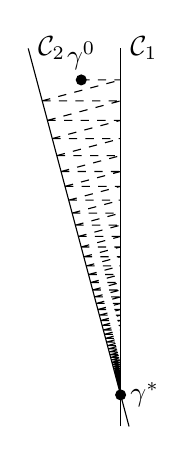
\begin{tikzpicture}
\fill (-0.500000,4.000000) circle (2pt) node[above] (gamma0) {$\gamma^0$};
\fill (0,0) circle (2pt) node[right] {$\gamma^*$};
\draw[dashed] (-0.500000,4.000000) -- (0.000000,4.000000)
(-0.995851,3.734440) -- (0.000000,4.000000)
(-0.995851,3.734440) -- (0.000000,3.734440)
(-0.929736,3.486510) -- (0.000000,3.734440)
(-0.929736,3.486510) -- (0.000000,3.486510)
(-0.868011,3.255041) -- (0.000000,3.486510)
(-0.868011,3.255041) -- (0.000000,3.255041)
(-0.810384,3.038938) -- (0.000000,3.255041)
(-0.810384,3.038938) -- (0.000000,3.038938)
(-0.756582,2.837183) -- (0.000000,3.038938)
(-0.756582,2.837183) -- (0.000000,2.837183)
(-0.706353,2.648822) -- (0.000000,2.837183)
(-0.706353,2.648822) -- (0.000000,2.648822)
(-0.659458,2.472967) -- (0.000000,2.648822)
(-0.659458,2.472967) -- (0.000000,2.472967)
(-0.615676,2.308787) -- (0.000000,2.472967)
(-0.615676,2.308787) -- (0.000000,2.308787)
(-0.574802,2.155506) -- (0.000000,2.308787)
(-0.574802,2.155506) -- (0.000000,2.155506)
(-0.536641,2.012402) -- (0.000000,2.155506)
(-0.536641,2.012402) -- (0.000000,2.012402)
(-0.501013,1.878799) -- (0.000000,2.012402)
(-0.501013,1.878799) -- (0.000000,1.878799)
(-0.467751,1.754065) -- (0.000000,1.878799)
(-0.467751,1.754065) -- (0.000000,1.754065)
(-0.436697,1.637613) -- (0.000000,1.754065)
(-0.436697,1.637613) -- (0.000000,1.637613)
(-0.407704,1.528891) -- (0.000000,1.637613)
(-0.407704,1.528891) -- (0.000000,1.528891)
(-0.380637,1.427388) -- (0.000000,1.528891)
(-0.380637,1.427388) -- (0.000000,1.427388)
(-0.355366,1.332624) -- (0.000000,1.427388)
(-0.355366,1.332624) -- (0.000000,1.332624)
(-0.331774,1.244151) -- (0.000000,1.332624)
(-0.331774,1.244151) -- (0.000000,1.244151)
(-0.309747,1.161552) -- (0.000000,1.244151)
(-0.309747,1.161552) -- (0.000000,1.161552)
(-0.289183,1.084436) -- (0.000000,1.161552)
(-0.289183,1.084436) -- (0.000000,1.084436)
(-0.269984,1.012440) -- (0.000000,1.084436)
(-0.269984,1.012440) -- (0.000000,1.012440)
(-0.252060,0.945225) -- (0.000000,1.012440)
(-0.252060,0.945225) -- (0.000000,0.945225)
(-0.235326,0.882471) -- (0.000000,0.945225)
(-0.235326,0.882471) -- (0.000000,0.882471)
(-0.219702,0.823884) -- (0.000000,0.882471)
(-0.219702,0.823884) -- (0.000000,0.823884)
(-0.205116,0.769186) -- (0.000000,0.823884)
(-0.205116,0.769186) -- (0.000000,0.769186)
(-0.191499,0.718120) -- (0.000000,0.769186)
(-0.191499,0.718120) -- (0.000000,0.718120)
(-0.178785,0.670444) -- (0.000000,0.718120)
(-0.178785,0.670444) -- (0.000000,0.670444)
(-0.166915,0.625933) -- (0.000000,0.670444)
(-0.166915,0.625933) -- (0.000000,0.625933)
(-0.155834,0.584377) -- (0.000000,0.625933)
(-0.155834,0.584377) -- (0.000000,0.584377)
(-0.145488,0.545580) -- (0.000000,0.584377)
(-0.145488,0.545580) -- (0.000000,0.545580)
(-0.135829,0.509359) -- (0.000000,0.545580)
(-0.135829,0.509359) -- (0.000000,0.509359)
(-0.126811,0.475543) -- (0.000000,0.509359)
(-0.126811,0.475543) -- (0.000000,0.475543)
(-0.118392,0.443972) -- (0.000000,0.475543)
(-0.118392,0.443972) -- (0.000000,0.443972)
(-0.110532,0.414496) -- (0.000000,0.443972)
(-0.110532,0.414496) -- (0.000000,0.414496)
(-0.103194,0.386978) -- (0.000000,0.414496)
(-0.103194,0.386978) -- (0.000000,0.386978)
(-0.096343,0.361286) -- (0.000000,0.386978)
(-0.096343,0.361286) -- (0.000000,0.361286)
(-0.089947,0.337301) -- (0.000000,0.361286)
(-0.089947,0.337301) -- (0.000000,0.337301)
(-0.083975,0.314907) -- (0.000000,0.337301)
(-0.083975,0.314907) -- (0.000000,0.314907)
(-0.078400,0.294000) -- (0.000000,0.314907)
(-0.078400,0.294000) -- (0.000000,0.294000)
(-0.073195,0.274482) -- (0.000000,0.294000)
(-0.073195,0.274482) -- (0.000000,0.274482)
(-0.068336,0.256259) -- (0.000000,0.274482)
(-0.068336,0.256259) -- (0.000000,0.256259)
(-0.063799,0.239246) -- (0.000000,0.256259)
(-0.063799,0.239246) -- (0.000000,0.239246)
(-0.059563,0.223362) -- (0.000000,0.239246)
(-0.059563,0.223362) -- (0.000000,0.223362)
(-0.055609,0.208533) -- (0.000000,0.223362)
(-0.055609,0.208533) -- (0.000000,0.208533)
(-0.051917,0.194689) -- (0.000000,0.208533)
(-0.051917,0.194689) -- (0.000000,0.194689)
(-0.048470,0.181763) -- (0.000000,0.194689)
(-0.048470,0.181763) -- (0.000000,0.181763)
(-0.045252,0.169696) -- (0.000000,0.181763)
(-0.045252,0.169696) -- (0.000000,0.169696)
(-0.042248,0.158430) -- (0.000000,0.169696)
(-0.042248,0.158430) -- (0.000000,0.158430)
(-0.039443,0.147912) -- (0.000000,0.158430)
(-0.039443,0.147912) -- (0.000000,0.147912)
(-0.036825,0.138092) -- (0.000000,0.147912)
(-0.036825,0.138092) -- (0.000000,0.138092)
(-0.034380,0.128924) -- (0.000000,0.138092)
(-0.034380,0.128924) -- (0.000000,0.128924)
(-0.032097,0.120365) -- (0.000000,0.128924)
(-0.032097,0.120365) -- (0.000000,0.120365)
(-0.029966,0.112374) -- (0.000000,0.120365)
(-0.029966,0.112374) -- (0.000000,0.112374)
(-0.027977,0.104913) -- (0.000000,0.112374)
(-0.027977,0.104913) -- (0.000000,0.104913)
(-0.026119,0.097948) -- (0.000000,0.104913)
(-0.026119,0.097948) -- (0.000000,0.097948)
(-0.024385,0.091445) -- (0.000000,0.097948)
(-0.024385,0.091445) -- (0.000000,0.091445)
(-0.022766,0.085374) -- (0.000000,0.091445)
(-0.022766,0.085374) -- (0.000000,0.085374)
(-0.021255,0.079706) -- (0.000000,0.085374)
(-0.021255,0.079706) -- (0.000000,0.079706)
(-0.019844,0.074415) -- (0.000000,0.079706)
(-0.019844,0.074415) -- (0.000000,0.074415)
(-0.018526,0.069474) -- (0.000000,0.074415)
(-0.018526,0.069474) -- (0.000000,0.069474)
(-0.017296,0.064862) -- (0.000000,0.069474)
(-0.017296,0.064862) -- (0.000000,0.064862)
(-0.016148,0.060556) -- (0.000000,0.064862)
(-0.016148,0.060556) -- (0.000000,0.060556)
(-0.015076,0.056535) -- (0.000000,0.060556)
(-0.015076,0.056535) -- (0.000000,0.056535)
(-0.014075,0.052782) -- (0.000000,0.056535)
(-0.014075,0.052782) -- (0.000000,0.052782)
(-0.013141,0.049278) -- (0.000000,0.052782)
(-0.013141,0.049278) -- (0.000000,0.049278)
(-0.012268,0.046006) -- (0.000000,0.049278)
(-0.012268,0.046006) -- (0.000000,0.046006)
(-0.011454,0.042952) -- (0.000000,0.046006)
(-0.011454,0.042952) -- (0.000000,0.042952)
(-0.010693,0.040100) -- (0.000000,0.042952)
(-0.010693,0.040100) -- (0.000000,0.040100)
(-0.009983,0.037438) -- (0.000000,0.040100)
(-0.009983,0.037438) -- (0.000000,0.037438)
(-0.009321,0.034952) -- (0.000000,0.037438)
(-0.009321,0.034952) -- (0.000000,0.034952)
(-0.008702,0.032632) -- (0.000000,0.034952)
(-0.008702,0.032632) -- (0.000000,0.032632)
(-0.008124,0.030466) -- (0.000000,0.032632)
(-0.008124,0.030466) -- (0.000000,0.030466)
(-0.007585,0.028443) -- (0.000000,0.030466)
(-0.007585,0.028443) -- (0.000000,0.028443)
(-0.007081,0.026555) -- (0.000000,0.028443)
(-0.007081,0.026555) -- (0.000000,0.026555)
(-0.006611,0.024792) -- (0.000000,0.026555)
(-0.006611,0.024792) -- (0.000000,0.024792)
(-0.006172,0.023146) -- (0.000000,0.024792)
(-0.006172,0.023146) -- (0.000000,0.023146)
(-0.005762,0.021609) -- (0.000000,0.023146)
(-0.005762,0.021609) -- (0.000000,0.021609)
(-0.005380,0.020174) -- (0.000000,0.021609)
(-0.005380,0.020174) -- (0.000000,0.020174)
(-0.005023,0.018835) -- (0.000000,0.020174)
(-0.005023,0.018835) -- (0.000000,0.018835)
(-0.004689,0.017585) -- (0.000000,0.018835)
(-0.004689,0.017585) -- (0.000000,0.017585)
(-0.004378,0.016417) -- (0.000000,0.017585)
(-0.004378,0.016417) -- (0.000000,0.016417)
(-0.004087,0.015327) -- (0.000000,0.016417)
(-0.004087,0.015327) -- (0.000000,0.015327)
(-0.003816,0.014310) -- (0.000000,0.015327)
(-0.003816,0.014310) -- (0.000000,0.014310)
(-0.003563,0.013360) -- (0.000000,0.014310)
(-0.003563,0.013360) -- (0.000000,0.013360)
(-0.003326,0.012473) -- (0.000000,0.013360)
(-0.003326,0.012473) -- (0.000000,0.012473)
(-0.003105,0.011645) -- (0.000000,0.012473)
(-0.003105,0.011645) -- (0.000000,0.011645)
(-0.002899,0.010872) -- (0.000000,0.011645)
(-0.002899,0.010872) -- (0.000000,0.010872)
(-0.002707,0.010150) -- (0.000000,0.010872)
(-0.002707,0.010150) -- (0.000000,0.010150)
(-0.002527,0.009476) -- (0.000000,0.010150)
(-0.002527,0.009476) -- (0.000000,0.009476)
(-0.002359,0.008847) -- (0.000000,0.009476)
(-0.002359,0.008847) -- (0.000000,0.008847)
(-0.002203,0.008259) -- (0.000000,0.008847)
(-0.002203,0.008259) -- (0.000000,0.008259)
(-0.002056,0.007711) -- (0.000000,0.008259)
(-0.002056,0.007711) -- (0.000000,0.007711)
(-0.001920,0.007199) -- (0.000000,0.007711)
(-0.001920,0.007199) -- (0.000000,0.007199)
(-0.001792,0.006721) -- (0.000000,0.007199)
(-0.001792,0.006721) -- (0.000000,0.006721)
(-0.001673,0.006275) -- (0.000000,0.006721)
(-0.001673,0.006275) -- (0.000000,0.006275)
(-0.001562,0.005858) -- (0.000000,0.006275)
(-0.001562,0.005858) -- (0.000000,0.005858)
(-0.001459,0.005469) -- (0.000000,0.005858)
(-0.001459,0.005469) -- (0.000000,0.005469)
(-0.001362,0.005106) -- (0.000000,0.005469)
(-0.001362,0.005106) -- (0.000000,0.005106)
(-0.001271,0.004767) -- (0.000000,0.005106)
(-0.001271,0.004767) -- (0.000000,0.004767)
(-0.001187,0.004451) -- (0.000000,0.004767)
(-0.001187,0.004451) -- (0.000000,0.004451)
(-0.001108,0.004155) -- (0.000000,0.004451)
;
\draw (-0.000000,-0.400000) -- (0.000000,4.400000) node[right] {$\mathcal{C}_1$};
\draw (0.106667,-0.400000) -- (-1.173333,4.400000) node[right] {$\mathcal{C}_2$};
\end{tikzpicture}
&
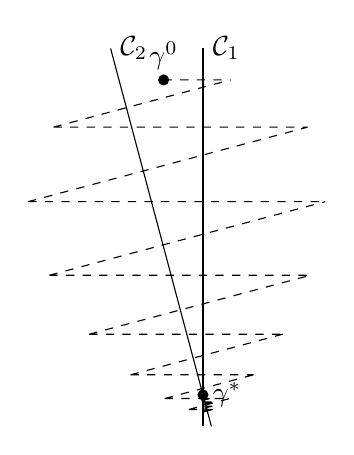
\begin{tikzpicture}
\fill (-0.500000,4.000000) circle (2pt) node[above] (gamma0) {$\gamma^0$};
\fill (0,0) circle (2pt) node[right] {$\gamma^*$};
\draw[dashed] (-0.500000,4.000000) -- (0.350000,4.000000)
(-1.898444,3.400415) -- (0.350000,4.000000)
(-1.898444,3.400415) -- (1.328911,3.400415)
(-2.219432,2.454190) -- (1.328911,3.400415)
(-2.219432,2.454190) -- (1.553603,2.454190)
(-1.950880,1.519661) -- (1.553603,2.454190)
(-1.950880,1.519661) -- (1.365616,1.519661)
(-1.444980,0.770169) -- (1.365616,1.519661)
(-1.444980,0.770169) -- (1.011486,0.770169)
(-0.919844,0.255148) -- (1.011486,0.770169)
(-0.919844,0.255148) -- (0.643891,0.255148)
(-0.486040,-0.046167) -- (0.643891,0.255148)
(-0.486040,-0.046167) -- (0.340228,-0.046167)
(-0.180221,-0.184954) -- (0.340228,-0.046167)
(-0.180221,-0.184954) -- (0.126154,-0.184954)
(0.004209,-0.217472) -- (0.126154,-0.184954)
(0.004209,-0.217472) -- (-0.002946,-0.217472)
(0.093772,-0.191681) -- (-0.002946,-0.217472)
(0.093772,-0.191681) -- (-0.065641,-0.191681)
(0.119666,-0.142266) -- (-0.065641,-0.191681)
(0.119666,-0.142266) -- (-0.083766,-0.142266)
(0.109394,-0.090756) -- (-0.083766,-0.142266)
(0.109394,-0.090756) -- (-0.076576,-0.090756)
(0.083372,-0.048103) -- (-0.076576,-0.090756)
(0.083372,-0.048103) -- (-0.058360,-0.048103)
(0.054625,-0.017974) -- (-0.058360,-0.048103)
(0.054625,-0.017974) -- (-0.038237,-0.017974)
(0.030058,0.000238) -- (-0.038237,-0.017974)
(0.030058,0.000238) -- (-0.021040,0.000238)
(0.012253,0.009116) -- (-0.021040,0.000238)
(0.012253,0.009116) -- (-0.008577,0.009116)
(0.001178,0.011717) -- (-0.008577,0.009116)
(0.001178,0.011717) -- (-0.000824,0.011717)
(-0.004475,0.010744) -- (-0.000824,0.011717)
(-0.004475,0.010744) -- (0.003133,0.010744)
(-0.006387,0.008205) -- (0.003133,0.010744)
(-0.006387,0.008205) -- (0.004471,0.008205)
(-0.006098,0.005387) -- (0.004471,0.008205)
(-0.006098,0.005387) -- (0.004268,0.005387)
(-0.004786,0.002973) -- (0.004268,0.005387)
(-0.004786,0.002973) -- (0.003350,0.002973)
(-0.003225,0.001219) -- (0.003350,0.002973)
(-0.003225,0.001219) -- (0.002258,0.001219)
(-0.001842,0.000126) -- (0.002258,0.001219)
(-0.001842,0.000126) -- (0.001289,0.000126)
(-0.000810,-0.000434) -- (0.001289,0.000126)
(-0.000810,-0.000434) -- (0.000567,-0.000434)
(-0.000149,-0.000625) -- (0.000567,-0.000434)
(-0.000149,-0.000625) -- (0.000105,-0.000625)
(0.000203,-0.000599) -- (0.000105,-0.000625)
(0.000203,-0.000599) -- (-0.000142,-0.000599)
(0.000337,-0.000471) -- (-0.000142,-0.000599)
(0.000337,-0.000471) -- (-0.000236,-0.000471)
(0.000338,-0.000318) -- (-0.000236,-0.000471)
(0.000338,-0.000318) -- (-0.000236,-0.000318)
(0.000273,-0.000182) -- (-0.000236,-0.000318)
(0.000273,-0.000182) -- (-0.000191,-0.000182)
(0.000189,-0.000080) -- (-0.000191,-0.000182)
(0.000189,-0.000080) -- (-0.000133,-0.000080)
(0.000112,-0.000015) -- (-0.000133,-0.000080)
(0.000112,-0.000015) -- (-0.000078,-0.000015)
(0.000052,0.000020) -- (-0.000078,-0.000015)
(0.000052,0.000020) -- (-0.000037,0.000020)
(0.000013,0.000033) -- (-0.000037,0.000020)
(0.000013,0.000033) -- (-0.000009,0.000033)
(-0.000008,0.000033) -- (-0.000009,0.000033)
(-0.000008,0.000033) -- (0.000006,0.000033)
(-0.000018,0.000027) -- (0.000006,0.000033)
(-0.000018,0.000027) -- (0.000012,0.000027)
(-0.000019,0.000019) -- (0.000012,0.000027)
(-0.000019,0.000019) -- (0.000013,0.000019)
(-0.000016,0.000011) -- (0.000013,0.000019)
(-0.000016,0.000011) -- (0.000011,0.000011)
(-0.000011,0.000005) -- (0.000011,0.000011)
(-0.000011,0.000005) -- (0.000008,0.000005)
(-0.000007,0.000001) -- (0.000008,0.000005)
(-0.000007,0.000001) -- (0.000005,0.000001)
(-0.000003,-0.000001) -- (0.000005,0.000001)
(-0.000003,-0.000001) -- (0.000002,-0.000001)
(-0.000001,-0.000002) -- (0.000002,-0.000001)
(-0.000001,-0.000002) -- (0.000001,-0.000002)
(0.000000,-0.000002) -- (0.000001,-0.000002)
(0.000000,-0.000002) -- (-0.000000,-0.000002)
(0.000001,-0.000002) -- (-0.000000,-0.000002)
(0.000001,-0.000002) -- (-0.000001,-0.000002)
(0.000001,-0.000001) -- (-0.000001,-0.000002)
(0.000001,-0.000001) -- (-0.000001,-0.000001)
(0.000001,-0.000001) -- (-0.000001,-0.000001)
(0.000001,-0.000001) -- (-0.000001,-0.000001)
(0.000001,-0.000000) -- (-0.000001,-0.000001)
(0.000001,-0.000000) -- (-0.000000,-0.000000)
(0.000000,-0.000000) -- (-0.000000,-0.000000)
(0.000000,-0.000000) -- (-0.000000,-0.000000)
(0.000000,0.000000) -- (-0.000000,-0.000000)
(0.000000,0.000000) -- (-0.000000,0.000000)
(0.000000,0.000000) -- (-0.000000,0.000000)
(0.000000,0.000000) -- (-0.000000,0.000000)
(-0.000000,0.000000) -- (-0.000000,0.000000)
(-0.000000,0.000000) -- (0.000000,0.000000)
(-0.000000,0.000000) -- (0.000000,0.000000)
(-0.000000,0.000000) -- (0.000000,0.000000)
(-0.000000,0.000000) -- (0.000000,0.000000)
(-0.000000,0.000000) -- (0.000000,0.000000)
(-0.000000,0.000000) -- (0.000000,0.000000)
(-0.000000,0.000000) -- (0.000000,0.000000)
(-0.000000,0.000000) -- (0.000000,0.000000)
(-0.000000,0.000000) -- (0.000000,0.000000)
(-0.000000,0.000000) -- (0.000000,0.000000)
(-0.000000,0.000000) -- (0.000000,0.000000)
(-0.000000,-0.000000) -- (0.000000,0.000000)
(-0.000000,-0.000000) -- (0.000000,-0.000000)
(-0.000000,-0.000000) -- (0.000000,-0.000000)
(-0.000000,-0.000000) -- (0.000000,-0.000000)
(-0.000000,-0.000000) -- (0.000000,-0.000000)
(-0.000000,-0.000000) -- (0.000000,-0.000000)
(0.000000,-0.000000) -- (0.000000,-0.000000)
(0.000000,-0.000000) -- (-0.000000,-0.000000)
(0.000000,-0.000000) -- (-0.000000,-0.000000)
(0.000000,-0.000000) -- (-0.000000,-0.000000)
(0.000000,-0.000000) -- (-0.000000,-0.000000)
(0.000000,-0.000000) -- (-0.000000,-0.000000)
(0.000000,-0.000000) -- (-0.000000,-0.000000)
(0.000000,-0.000000) -- (-0.000000,-0.000000)
(0.000000,-0.000000) -- (-0.000000,-0.000000)
(0.000000,-0.000000) -- (-0.000000,-0.000000)
(0.000000,-0.000000) -- (-0.000000,-0.000000)
(0.000000,-0.000000) -- (-0.000000,-0.000000)
(0.000000,0.000000) -- (-0.000000,-0.000000)
(0.000000,0.000000) -- (-0.000000,0.000000)
(0.000000,0.000000) -- (-0.000000,0.000000)
(0.000000,0.000000) -- (-0.000000,0.000000)
(-0.000000,0.000000) -- (-0.000000,0.000000)
(-0.000000,0.000000) -- (0.000000,0.000000)
(-0.000000,0.000000) -- (0.000000,0.000000)
(-0.000000,0.000000) -- (0.000000,0.000000)
(-0.000000,0.000000) -- (0.000000,0.000000)
(-0.000000,0.000000) -- (0.000000,0.000000)
(-0.000000,0.000000) -- (0.000000,0.000000)
(-0.000000,0.000000) -- (0.000000,0.000000)
(-0.000000,0.000000) -- (0.000000,0.000000)
(-0.000000,0.000000) -- (0.000000,0.000000)
(-0.000000,0.000000) -- (0.000000,0.000000)
(-0.000000,0.000000) -- (0.000000,0.000000)
(-0.000000,-0.000000) -- (0.000000,0.000000)
(-0.000000,-0.000000) -- (0.000000,-0.000000)
(-0.000000,-0.000000) -- (0.000000,-0.000000)
(-0.000000,-0.000000) -- (0.000000,-0.000000)
(0.000000,-0.000000) -- (0.000000,-0.000000)
(0.000000,-0.000000) -- (-0.000000,-0.000000)
(0.000000,-0.000000) -- (-0.000000,-0.000000)
(0.000000,-0.000000) -- (-0.000000,-0.000000)
(0.000000,-0.000000) -- (-0.000000,-0.000000)
(0.000000,-0.000000) -- (-0.000000,-0.000000)
(0.000000,-0.000000) -- (-0.000000,-0.000000)
(0.000000,-0.000000) -- (-0.000000,-0.000000)
(0.000000,-0.000000) -- (-0.000000,-0.000000)
(0.000000,-0.000000) -- (-0.000000,-0.000000)
(0.000000,-0.000000) -- (-0.000000,-0.000000)
(0.000000,-0.000000) -- (-0.000000,-0.000000)
(0.000000,0.000000) -- (-0.000000,-0.000000)
(0.000000,0.000000) -- (-0.000000,0.000000)
(0.000000,0.000000) -- (-0.000000,0.000000)
(0.000000,0.000000) -- (-0.000000,0.000000)
(-0.000000,0.000000) -- (-0.000000,0.000000)
(-0.000000,0.000000) -- (0.000000,0.000000)
(-0.000000,0.000000) -- (0.000000,0.000000)
(-0.000000,0.000000) -- (0.000000,0.000000)
(-0.000000,0.000000) -- (0.000000,0.000000)
(-0.000000,0.000000) -- (0.000000,0.000000)
(-0.000000,0.000000) -- (0.000000,0.000000)
(-0.000000,0.000000) -- (0.000000,0.000000)
(-0.000000,0.000000) -- (0.000000,0.000000)
(-0.000000,0.000000) -- (0.000000,0.000000)
(-0.000000,0.000000) -- (0.000000,0.000000)
(-0.000000,0.000000) -- (0.000000,0.000000)
(-0.000000,-0.000000) -- (0.000000,0.000000)
(-0.000000,-0.000000) -- (0.000000,-0.000000)
(-0.000000,-0.000000) -- (0.000000,-0.000000)
(-0.000000,-0.000000) -- (0.000000,-0.000000)
(0.000000,-0.000000) -- (0.000000,-0.000000)
(0.000000,-0.000000) -- (-0.000000,-0.000000)
(0.000000,-0.000000) -- (-0.000000,-0.000000)
(0.000000,-0.000000) -- (-0.000000,-0.000000)
(0.000000,-0.000000) -- (-0.000000,-0.000000)
(0.000000,-0.000000) -- (-0.000000,-0.000000)
(0.000000,-0.000000) -- (-0.000000,-0.000000)
(0.000000,-0.000000) -- (-0.000000,-0.000000)
(0.000000,-0.000000) -- (-0.000000,-0.000000)
(0.000000,-0.000000) -- (-0.000000,-0.000000)
(0.000000,-0.000000) -- (-0.000000,-0.000000)
(0.000000,-0.000000) -- (-0.000000,-0.000000)
(0.000000,0.000000) -- (-0.000000,-0.000000)
(0.000000,0.000000) -- (-0.000000,0.000000)
(0.000000,0.000000) -- (-0.000000,0.000000)
(0.000000,0.000000) -- (-0.000000,0.000000)
(0.000000,0.000000) -- (-0.000000,0.000000)
(0.000000,0.000000) -- (-0.000000,0.000000)
(-0.000000,0.000000) -- (-0.000000,0.000000)
(-0.000000,0.000000) -- (0.000000,0.000000)
(-0.000000,0.000000) -- (0.000000,0.000000)
;
\draw (-0.000000,-0.400000) -- (0.000000,4.400000) node[right] {$\mathcal{C}_1$};
\draw (0.106667,-0.400000) -- (-1.173333,4.400000) node[right] {$\mathcal{C}_2$};
\end{tikzpicture}
\\
(a)&(b)&(c)
\end{tabular}
\caption{\label{alternate_projections} The trajectory of $\gamma^l$ given by the Sinkhorn algorithm is illustrated for decreasing values of $\epsilon$ in (a) and (b). In order to accelerate the convergence rate, over-relaxed projections are here considered (c).}
\end{center}
\end{figure}
\subsection{Over-relaxed projections}

Let us define the $\omega$-over-relaxed projection operator by:
\begin{equation}\label{eq:def_or_proj}
\log P^\omega_{\Ccal_k}(\gamma) = (1-\omega) \log \gamma + \omega \log P_{\Ccal_k}(\gamma),
\end{equation}
where the logarithm is taken coordinate-wise.
Note that $P_{\Ccal_k}^0 = Id$, $P_{\Ccal_k}^1 = P_{\Ccal_k}$ gives the Sinkhorn algorithm, and $P_{\Ccal_k}^2$ is an involution (this is non-trivial, and uses the fact that $\Ccal_k$ is an affine subspace).

{\color{blue} \begin{proposition} 
State here that the fixed points of   $\gamma^{l+1} =P^\theta_{\Ccal_2}(P^\theta_{\Ccal_1}(\gamma^l))$ are the same than $\gamma^{l+1} =P_{\Ccal_2}(P_{\Ccal_1}(\gamma^l))$?
\end{proposition}}
\subsection{Lyapunov function}
Let $\gamma^*$ denote the solution of the regularized OT problem.
The function $F$ is defined as:
\begin{equation}\label{eq:lyapunov_function}
F(\gamma) = KL(\gamma^*, \gamma)
\end{equation}
It shall be used as a Lyapunov function, so that $F(\gamma^{k+1}) < F(\gamma^k)$ as long as the process has not converged.

We argue that it makes sense to consider this Lyapunov function.
Obviously, it is closely related to the notion of Bregman projection that is used throughout the algorithm.
But it is also easy to calculate its decrease, as shown in lemma \ref{lemma:lyapunov_decrease}.
Moreover, in practice it allows the use of a wide range of over-relaxation parameters.

\begin{lemma} \label{lemma:KL_compact}
	For any $M \in \IR_+^*$, the sublevel set $K := \left\{ \gamma \mid F(\gamma) \le M \right\}$ is compact.
\end{lemma}
\begin{proof}
	First note that K is closed in $\IR_{+*}^{n_1 n_2}$, by continuity of $F$.
	For $\gamma \in K$, one has:
	\begin{align*}
	F(\gamma) &= \scal{\gamma^*}{\log \gamma^* - 1} + \scal{\gamma}{1} - \scal{\gamma^*}{\log \gamma}\\
	\sum_{i,j} \gamma_{i,j} - \gamma^*_{i,j} \log \gamma_{i,j} &\le M - \scal{\gamma^*}{\log \gamma^* - 1} .
	\end{align*}
	By concavity, the logarithm admits a simple upper bound: $\log \gamma_{i,j} \le \frac{\gamma_{i,j}}{e}$. Moreover, since $\gamma^*$ is a solution of the problem, each of its coordinates is at most 1.
	\begin{align*}
	\sum_{i,j} \gamma_{i,j} &\le \frac{M - \scal{\gamma^*}{\log \gamma^*-1}}{1-\frac{1}{e}} =: M'.
	\end{align*}
	Therefore each coordinate $\gamma_{i,j}$ is bounded above by $M'$.
	
	Let us show that the coordinates are bounded below by a strictly positive number; from which it can be deduced that $K$ is bounded and closed in $\IR^{n_1 n_2}$, and therefore compact.
	\begin{align*}
	F(\gamma)
	&\ge \scal{\gamma^*}{\log \gamma^*} - \sum_{i,j} \gamma^*_{i,j} \log(\gamma_{i,j}) - 1\\
	&\ge \scal{\gamma^*}{\log \gamma^*} - \gamma^*_{i_0,j_0} \log(\gamma_{i_0,j_0}) - 1 - \log M',
	\end{align*}
	where the last equation derives from $\log(y_{i,j}) \le \log M'$, and $\sum_{(i,j)\neq(i_0,j_0)} \gamma^*_{i,j} \le 1$.
	Finally:
	\[
	\log(\gamma_{i_0,j_0}) \ge \frac{\scal{\gamma^*}{\log \gamma^*} - M - \log M' - 1}{\gamma^*_{i_0,j_0}},
	\]
	and $K$ is thus compact.
\end{proof}


Note that the difference $F(\gamma) - F(P^\omega_{\Ccal_k}(\gamma))$ may be calculated without knowing $\gamma^*$, as shown by the following lemma.
\begin{lemma}\label{lemma:lyapunov_decrease}
	Take $\gamma$ in $\IR^{mn}_{+*}$. The decrease in value of the Lyapunov function can be calculated with the following formula:
	\begin{equation} \label{eq:kl_diff_scal}
	F(\gamma) - F(P^\omega_{\Ccal_k}(\gamma)) = 
	\scal{\mu^k}{\varphi_\omega \left(\frac{A_k \gamma}{\mu^k}\right)},
	\end{equation}
	where
	\begin{equation}
	\varphi_\omega(x) = x(1-x^{-\omega}) - \omega \log x
	\end{equation}
	is a real function, applied coordinate-wise.
\end{lemma}
\begin{proof}
From \eqref{KL}, we have $F(\gamma^1)-F(\gamma^2)= \sum_{i,j}\left(\gamma^*_{i,j}\log(\gamma^2_{i,j}/\gamma^1_{i,j})+\gamma^1_{i,j}-\gamma^2_{i,j}\right)$. The result can then be deduced from relations \eqref{eq:def_or_proj} and \eqref{scaling}.
\end{proof}
Thus,  the decrease in value of the function $F$ for a over-relaxed projection associated to $\Ccal_k$ is cheap to estimate, since its computational cost is  linear with respect to the dimension of data $\mu^k$. In Figure \ref{phi_omega}, we illustrate the functions  $\varphi_\omega$ for several values of $\omega$.
Notice that for the Sinkhorn algorithm, which corresponds to $\omega=1$, the function $\varphi_\omega$ is always nonnegative. For other values $1\le\omega<2$, it is nonnegative for arguments close to 1.
\begin{figure}[ht!]
\begin{center}
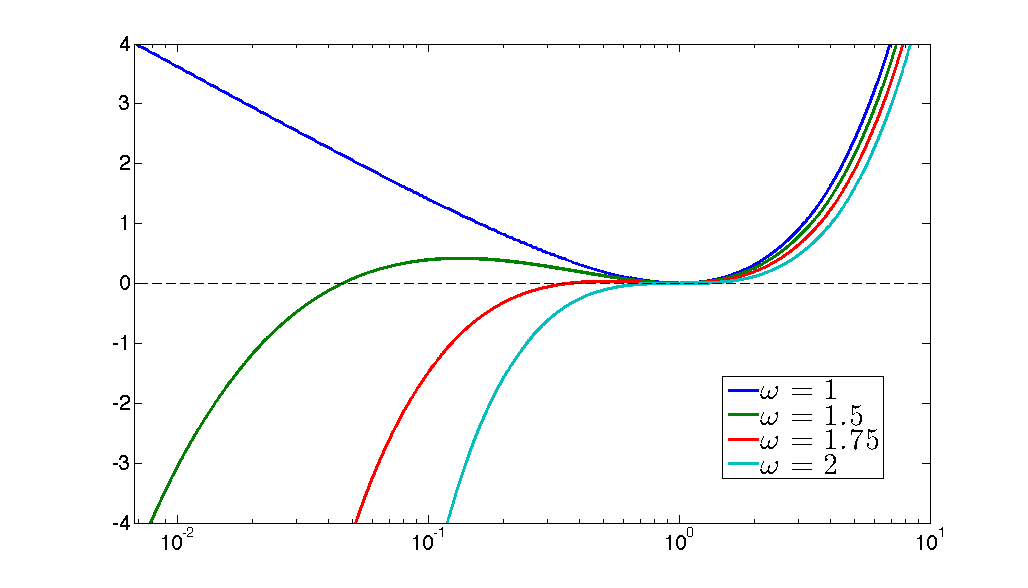
\includegraphics[width=11cm]{phi_omega.png}
\caption{\label{phi_omega} Plot of functions $\varphi_\omega(x)$ for different values $1\leq \omega\leq 2$ and   $x\in[10^{-2}, 10^1]$.}
\end{center}
\end{figure}
\subsection{Proposed algorithm}


\begin{theorem}\label{thm:algo}
	Let $\theta$ and $\omega$ be such that $1\le \theta < \omega < 2$. Let $U$ be the open set defined by:
	\begin{equation}\label{eq:open_set_U}
	U = \left\{
	\gamma \in \IR_{+*}^{nm} \mid
	F(P^\omega_{\Ccal_1}(\gamma)) < F(\gamma)
	\text{ and }
	F(P^\omega_{\Ccal_2}(P^\theta_{\Ccal_1}(\gamma))) < F(P^\theta_{\Ccal_1}(\gamma))
	\right\}.
	\end{equation}
	Set the initial value $\gamma^0 = e^{-c/\epsilon}$, and iterate:
	\begin{align*}
	\gamma^{l+1} =
	\begin{cases}
	P^\theta_{\Ccal_2}(P^\theta_{\Ccal_1}(\gamma^l)) & \text{if } \gamma \in U \\
	P_{\Ccal_2}(P_{\Ccal_1}(\gamma^l)) & \text{otherwise.}
	\end{cases}
	\end{align*}
	Then the iterates $(\gamma^l)$ converge to $\gamma^*$.
\end{theorem}
{\color{red} 
	In practice the test would be: check whether the $\omega$-relaxed projection of $\zeta$ on $\Ccal_1$ decreases the value of
	$F$; if so, calculate $P_{\Ccal_1}^\theta(\zeta)$ (don't update $\zeta$ yet) and check that its $\omega$-relaxed projection on $\Ccal_2$ decreases the value of $F$ again. \\
	$\longrightarrow$ Has to calculate 3 projections sometimes. This result is weaker than the one from my report, but easier to prove. Maybe we could avoid having $U$, and rather perform the test independently on each variable ? (Or we could find a cheaper test).}
\begin{remark}
	Given lemma \ref{lemma:lyapunov_decrease}, it can be seen that $\gamma^* \in U$. Therefore, iterations eventually all use the over-relaxed operators.
	
	
\end{remark}
{\color{blue} Comment: As the inequality is strict in U, $\gamma^*\notin U$.} 


\begin{lemma}[\cite{cuturi13}]
	\label{lemma:trivial_intersection}
	Let us take $\gamma^0$ in $\IR_{+*}^{n_1 n_2}$,
	and denote
	\[
	S = \left\{
	\diag(a) \gamma^0 \diag(b),\quad
	(a,b) \in \IR_{+*}^{n_1 + n_2}
	\right\}
	\]
	the set of matrices that are diagonally similar to $\gamma^0$.
	Then the set $S \cap \Ccal_1 \cap \Ccal_2$ contains exactly one element $\gamma^* = P_{\Ccal_1 \cap \Ccal_2}(\gamma^0)$.
\end{lemma}

\begin{lemma}\label{lemma:F_P_theta}
	Let $1\le \theta < \omega$. Then, for any $\gamma \in \IR_{+*}^{nm}$, one has
	\begin{equation}\label{eq:F_P_theta}
	F(P^\theta_{\Ccal_k}(\gamma)) \le F(P^\omega_{\Ccal_k}(\gamma)).
	\end{equation}
	Moreover, equality occurs if and only if $\gamma \in \Ccal_k$.
\end{lemma}
\begin{proof}
	Thanks to lemma \ref{lemma:lyapunov_decrease}, one knows that
	\[
	F(P^\theta_{\Ccal_k}(\gamma)) - F(P^\omega_{\Ccal_k}(\gamma))
	= \scal{\mu^k}{(\varphi_\omega - \varphi_\theta) \left( \frac{A_k \gamma}{\mu^k} \right) } .
	\]
	Moreover, $t \in [1,\infty) \mapsto \varphi_t(x)$ is nonincreasing:
	\[
	\frac{d}{dt} \varphi_t(x) = \log x (x^{1-t} - 1).
	\]
	For $x\neq 1$, it is even strictly decreasing.
	Thus the inequality (\ref{eq:F_P_theta}) is valid, with equality \emph{iff} $A_1 \gamma = \mu$.
\end{proof}

\begin{proof}[Proof of the theorem]
	First of all, notice that the operators $P_{\Ccal_k}^\theta$ apply a scaling to lines or columns of matrices. All $(\gamma^l)$ are thus diagonally similar to $\gamma^0$:
	\[
	\forall l\ge0,\quad \gamma^l \in S
	\]
	
	The set $U$ is constructed in such a way that, by applying lemma \ref{lemma:F_P_theta} several times, one ensures that the sequence $(F(\gamma^l))$ is nonincreasing. Moreover, it is strictly decreasing as long as $\gamma^l \not \in \Ccal_1 \cap \Ccal_2$.
	Hence, 
	\[
	F(\gamma^l) \le F(\gamma^0).
	\]
	By lemma \ref{lemma:KL_compact}, the sequence $(\gamma^l)$ is thus precompact. Let us show that any accumulation point $\zeta$ belongs to $\Ccal_1 \cap \Ccal_2$. Since $S$ is closed in $\IR_{+*}^{n_1 n_2}$, by lemma \ref{lemma:trivial_intersection} this would mean that $\zeta = \gamma^*$, and would be sufficient to prove the convergence.
	
	Let $(\gamma^{k_l})$ be a subsequence of $(\gamma^l)$ that converges to $\zeta$.
	Let us denote, for convenience, $T_1 = P_{\Ccal_2}^\theta \circ P_{\Ccal_1}^\theta$ and $T_2 = P_{\Ccal_2} \circ P_{\Ccal_1}$ the two operators used in the iteration, and $T$ the compound operator, so that $T_{|U} \equiv T_{1|U}$ and $T_{|U^c} \equiv T_{2|U^c}$.
	\begin{enumerate}[align=right,labelsep=10pt,leftmargin=0.5cm]
		\item[$\bullet$] If $\zeta \in U$, then since $U$ is open, all $(\gamma^{k_l})$ are eventually in $U$ as well.
		Thus, for any large enough $l$, $ T(\gamma^{k_l}) = T_1(\gamma^{k_l}) $. By continuity of $T_1$ on $U$, since $(\gamma^{k_l})$ converges to $\zeta$, 
		\[T(\zeta) = \lim_{l\rightarrow \infty} T(\gamma^{k_l}).\] Thus
		 \[F(T(\zeta)) = \lim_{l \rightarrow \infty} F(T(\gamma^{k_l})) \ge \lim_{l\rightarrow \infty} F(\gamma^{k_{l+1}}) .\]
		 \[
		 F(T(\zeta)) \ge F(\zeta)
		 \] Since $\zeta$ is inside the set $U$, which ensures strict decrease of the Lyapunov function, this is absurd.
		\item[$\bullet$] If $\zeta \in U^c$ and an infinite number of $(\gamma^{k_l})$ are in $U^c$, then the same argument of continuity applied to $T_2$ yields
		 \[
		 F(T(\zeta)) = F(\zeta).
		 \]
		 The function $\varphi_1$ from lemma \ref{lemma:lyapunov_decrease} is strictly positive except at $x=1$. Since the case of equality occurs for both projections, this ensures that $\zeta \in \Ccal_1 \cap \Ccal_2$.
		 
		 \item[$\bullet$] If $\zeta \in U^c$ and all but finitely many $\gamma^{k_l}$ are in $U$, then $\zeta$ is on the border $\partial U$. In particular it belongs to $\bar{U}$, and therefore
		 \[
		 F(P^\omega_{\Ccal_1}(\zeta)) \le F(\zeta) \quad
		 \text{ and } \quad
		 F(P^\omega_{\Ccal_2}(P^\theta_{\Ccal_1}(\zeta))) \le F(P^\theta_{\Ccal_1}(\zeta)).
		 \]
		 By lemma \ref{lemma:F_P_theta}, the inequality \begin{equation} \label{eq:ineq1}
		 F(P_{\Ccal_1}^\theta(\zeta)) \le F(P_{\Ccal_1}^\omega(\zeta)) \end{equation}
		 is valid; it is strict unless $\zeta \in \Ccal_1$.
		 The same lemma yields
		 \begin{equation} \label{eq:ineq2}
		 F(P_{\Ccal_2}^\theta(P_{\Ccal_1}^\theta(\zeta)) \le F(P_{\Ccal_2}^\omega(P_{\Ccal_1}^\theta(\zeta)), \end{equation}
		 with a strict inequality unless $P_{\Ccal_1}^\theta(\zeta) \in \Ccal_2$.
		 To sum up, we have the series of inequalities:
		 \[
		 F(\zeta) 
		 \overset{\zeta \in \bar{U}}{\ge}
		 F(P^\omega_{\Ccal_1}(\zeta))
		 \overset{\text{(\ref{eq:ineq1})}}{\ge}
		 F(P^\theta_{\Ccal_1}(\zeta))
		 \overset{\zeta \in U}{\ge}
		 F(P_{\Ccal_2}^\omega(P_{\Ccal_1}^\theta(\zeta)))
		 \overset{\text{(\ref{eq:ineq2})}}{\ge}
		 F(P_{\Ccal_2}^\theta(P_{\Ccal_1}^\theta(\zeta)))
		 \]
		 
		 Yet, by continuity of $T_1 = P_{\Ccal_2}^\theta \circ P_{\Ccal_1}^\theta $ on $\bar{U}$, we have
		 \[
		 F(P_{\Ccal_2}^\theta(P_{\Ccal_1}^\theta(\zeta))) = F(\zeta).
		 \]
		 Thus both (\ref{eq:ineq1}) and (\ref{eq:ineq2}) fall in the case of equality, which means $\zeta \in \Ccal_1$ and $P^\theta_{\Ccal_1}(\zeta) = \zeta \in \Ccal_2$.
	\end{enumerate}
\end{proof}


\section{Local rate of convergence ?}
Some material to adapt Lenaic results:


The Sinkhorn algorithm can be interpreted as an alternate maximisation algorithm on the dual of the regularized optimal transport problem.
The dual problem of \eqref{ROT} is:
\begin{equation}\label{DROT}\max_{\alpha,\beta}\langle \alpha,\mu^1\rangle+\langle \beta,\mu^2\rangle-\epsilon\sum_{i,j}e^{(\alpha_i+\beta_j-c_{i,j})/\epsilon}\end{equation}
It is concave and continuously differentiable for all $(a,b)\in\IR^{n_1+n_2}$. Alternate maximization then converges and we recover, for $a_i=e^{\alpha_i/\epsilon}$, $b_j=e^{\beta_j/\epsilon}$ and $\gamma^0_{i,j}=e^{-c_{i,j}/\epsilon}$:
\begin{align*}
a^{l+1} &= {\mu^1}\oslash{\gamma^0 b^l} &
b^{l+1} &= {\mu^2}\oslash{^t \gamma^0 a^{l+1}} 
\end{align*}

If $(\alpha^*,\beta^*)$ is a solution of \eqref{DROT}, then all the 
other optimum can be written as $(\alpha^*+\kappa,\beta^*-\kappa)$, which means that the problem admits a unique solution, up to a translation with constant $\kappa\in\IR$.


The Hessian matrix of the functional in \eqref{DROT} at point $(\alpha,\beta)$ reads, for $a_i=e^{\alpha_i/\epsilon}>0$ and $b_j=e^{\beta_j/\epsilon}>0$:


$$H(a,b)=\frac1\epsilon\begin{bmatrix}
\diag(a)\diag(\gamma^0 b)&\diag(a)\gamma^0 \diag(b)\\
\diag(b){^t\gamma^0} \diag(a)&\diag(^t\gamma^0a)\diag(b)
\end{bmatrix}.$$
Notice that 

$$H(a^*,b^*)=\frac1\epsilon\begin{bmatrix}
\diag(\mu^1)&\gamma^*\\
^t\gamma^*&\diag(\mu^2)
\end{bmatrix}.$$


The matrices $H(a,b)$  are positive semi-definite. They have only one $0$ eigenvalue associated to the eigenvetor $^t[\mathbf{1},-\mathbf{1}]$. 
Using Schur complement properties, one can then show that any matrix $T(a,b)=(\diag(a)\diag(\gamma^0 b))^{-1}\diag(a)\gamma^0\diag(b)(\diag(^t\gamma^0a)\diag(b))^{-1} \diag(b){^t\gamma^0}\diag(a)=(\diag(\gamma^0 b))^{-1}\gamma^0(\diag(^t\gamma^0a))^{-1} \diag(b){^t\gamma^0}\diag(a)$ is positive semi definite for $a,b>0$. Moreover, we can show that $T$ has a unique largest eigenvalue that is $1$ and is associated to the eigenvector $\mathbf{1}$. All the other eigenvalues belongs to the set $[0;1[$.


From experiments, it seems possible to design a good guess for $\omega$ from $c$ and $\epsilon$ only. 
    Denoting as $\lambda$ the second larger eigenvalue of $T(1,1)$, one can set 
    $\omega=\frac{2}{\lambda}(1-\sqrt{1-\lambda})$.
    
    
    
\section{Experimental results}


In practice, we observed that the algorithm introduced in Theorem \ref{thm:algo} can be simplified and it is sufficient to check $F(P^\omega_{\Ccal_2}(P^\omega_{\Ccal_1}(\gamma^l)))-F(\gamma^l)>0$ for performing the over-relaxed iterations with parameter $\omega$.
The cost of this test is linear with respect to the data dimension (i.e. $o(n_1+n_2)$).

\renewcommand{\algorithmiccomment}[1]{\hfill\bgroup(#1)\egroup}
\begin{algorithm}
\caption{Over-relaxed Sinkhorn algorithm}
\label{SOR}
\begin{algorithmic}
\REQUIRE $\mu^1\in \IR^{n_1}$, $\mu^2\in \IR^{n_2}$, $c\in \IR^{n_1\times n_2}_+$
\STATE Set $a=\mathbf{1}_{n_1}$, $b=\mathbf{1}_{n_2}$, $\gamma^0=e^{-c/\epsilon}$, $\omega\in[1;2[$ and $\eta>0$
\WHILE {$||a\otimes \gamma^0b-  \mu_1||>\eta$}
\STATE $\tilde a=\mu_1\oslash (\gamma^0 b)$,  $a_\omega=a^{1-\omega}\otimes \tilde a^\omega$
\STATE $\tilde b=\mu_2\oslash (^t\gamma^0  a_\omega)$
\IF{ $\langle \mu^1,\varphi_\omega(a\oslash\tilde a) \rangle +\langle \mu^2,\varphi_\omega(b\oslash\tilde b)\rangle>0$}
\STATE  $a=a_\omega$, $b=b^{1-\omega}\otimes \tilde b^\omega$\COMMENT{Over-relaxed Sinkhorn iteration}
\ELSE
\STATE $a=\tilde a$, $b=\mu_2\oslash (^t\gamma^0 a)$  \COMMENT{Sinkhorn iteration}
\ENDIF
\ENDWHILE
 \RETURN $\gamma=\diag(a)\gamma^0\diag(b)$
\end{algorithmic}
\end{algorithm}

\begin{algorithm}
\caption{Over-relaxed Sinkhorn algorithm 2}
\label{SOR}
\begin{algorithmic}
\REQUIRE $\mu^1\in \IR^{n_1}$, $\mu^2\in \IR^{n_2}$, $c\in \IR^{n_1\times n_2}_+$
\STATE Set $a=\mathbf{1}_{n_1}$, $b=\mathbf{1}_{n_2}$, $\gamma^0=e^{-c/\epsilon}$, $\omega\in[1;2[$ and $\eta>0$
\WHILE {$||a\otimes \gamma^0b-  \mu_1||>\eta$}
\STATE $\tilde a=\mu_1\oslash (\gamma^0 b)$, 
\IF{ $\langle \mu^1,\varphi_\omega(a\oslash\tilde a) \rangle>0$}
\STATE  $a=a^{1-\omega}\otimes \tilde a^\omega$\COMMENT{Over-relaxed Sinkhorn iteration}
\ELSE
\STATE $a=\tilde a$,\COMMENT{Sinkhorn iteration}
\ENDIF
\STATE $\tilde b=\mu_2\oslash (^t\gamma^0  a)$
\IF{ $\langle \mu^2,\varphi_\omega(b\oslash\tilde b) \rangle>0$}
\STATE  $b=b^{1-\omega}\otimes \tilde b^\omega$\COMMENT{Over-relaxed Sinkhorn iteration}
\ELSE
\STATE $b=\tilde b$,\COMMENT{Sinkhorn iteration}
\ENDIF
\ENDWHILE
 \RETURN $\gamma=\diag(a)\gamma^0\diag(b)$
\end{algorithmic}
\end{algorithm}



{\color{red} TODO}


\section{Conclusion and perspectives}
Contributions: 
cheap test, preliminary work for convergence results. Huge acceleration in practice.


Perspectives:
global convergence, how chosing $\omega$?, intensive numerical study with respect to other accelerarions methods\cite{2016arXiv160604133S,2017arXiv170509634A}.





\section*{Acknowledgments}
This study has been carried out with financial support from the French State, managed by the French National Research Agency (ANR) in the frame of the  GOTMI project (ANR-16-CE33-0010-01).

%\subsubsection*{References}

\bibliographystyle{apalike}
\bibliography{references}

\end{document}
